\documentclass[brudnopis]{xmgr}
%\usepackage{xcolor}
% Jeśli nowe rozdziały mają się zaczynać na stronach nieparzystych:
%\documentclass[openright]{xmgr}
% install minted package to highlight source code
\usepackage{minted}
\usepackage{amsrefs}
\usepackage{epigraph}
\selectlanguage{polish}
\usepackage{hyperref}
\renewcommand{\epigraphflush}{flushleft} %or center or night
\setlength\epigraphwidth{8cm}
\setlength\epigraphrule{1pt}
%\definecolor{niceGreen}{rgb}{0,0.6,0}
%%\definecolor{niceBlue}{rgb}{0.0,0,0.9}
%\definecolor{niceGrey}{rgb}{0.5,0.5,0.5}
%\definecolor{stress}{cmyk}{0,1,0.13,0} % RubineRed
%\definecolor{topic}{cmyk}{0.98,0.13,0,0.43} % MidnightBlue
\defaultfontfeatures{Scale=MatchLowercase}
\setmainfont[Numbers=OldStyle,Ligatures=TeX]{Minion Pro}
\setsansfont[Numbers=OldStyle,Ligatures=TeX]{Myriad Pro}
% for fontspec version < 2.0
%\setmainfont[Numbers=OldStyle,Mapping=tex-text]{Minion Pro}
% \setsansfont[Numbers=OldStyle,Mapping=tex-text]{Myriad Pro}
%\setmonofont[Scale=0.75]{Monaco}
% Opcjonalnie identyfikator dokumentu
% drukowany tylko z~włączoną opcją 'brudnopis':
\wersja {wersja wstępna [\ymdtoday]}
\author {Szymon Filipowicz}
\nralbumu {224\,621}
\email {}
\title {Rozwój umiejętności awatara w~grze wideo na
podstawie rozgrywek z~innym graczem}
\date {15.09.2018}
\miejsce {Gdańsk}
\opiekun {dr Wiesław Pawłowski}
% dodatkowe polecenia
%\renewcommand{\filename}[1]{\texttt{#1}}
%\emph{formatowania strukturalnego}.
\begin{document}
% streszczenie
\begin{abstract}
Na przestrzeni kilku dekad gry wideo przeszły długą drogę dynamicznego rozwoju, od Pong'a do symulacji podróży po
kosmosie z~proceduralnie generowaną przestrzenią i~spektakularnymi, realistycznymi
bitwami dla tysięcy osób biorących udział w tym samym czasie. 

Wraz z~wymaganiami odbiorców wzrasta także poziom zaawansowania technologicznego. Zaczynają powstawać gry wykorzystujące sieci neuronowe, nauczanie maszynowe czy też przetwarzanie ogromnych zasobów danych w~czasie rzeczywistym. Próbą wykorzystania nowoczesnych mechanik jest projekt stworzony na potrzeby tej pracy.
\end{abstract}
% słowa kluczowe
\keywords{gra wideo,
C\#,
Unity3D,
nauczanie maszynowe,
strumienie danych}
% tytuł i~spis treści
\maketitle
% wstęp
\introduction

Gry powstały wraz z możliwościami technologicznymi. Początkowo programy rozrywkowe musiały dostosowywać się do sprzętu. Wiele lat później, związek ten stał się dużo bardziej równorzędny. Z~jednej strony zaczął powstawać i rozwijać się niezależnie sprzęt ściśle przeznaczony do grania. Natomiast z~drugiej strony, nie zapominając o swoich korzeniach, gdy tylko pojawiają się nowe technologie, firmy z branży gier wideo starają się jak najszybciej implementować je w swoim oprogramowaniu. Gdy gry starają się wykorzystywać nowy sprzęt i technologie, inne branże zaczęły starać się wykorzystywać właśnie gry.

Można to zauważyć w~zupełnie odmiennych niż IT branżach. Rozwiązania wymyślone na potrzeby gier mają coraz szersze zastosowanie w~życiu codziennym. Przykładem może być oprogramowanie edukacyjne czy systemy nagród oparte o tzw. grywalizację w~firmach. W~niniejszej pracy szczególna
uwaga zostanie zwrócona na zastosowaniu sztucznej inteligencji w~grach.

\chapter{Wprowadzenie do gier wideo}
Uznawana za pierwszą grę wideo ,,Pong'' (1972) rozpoczęła zupełnie
nowy nurt w~programowaniu. Nurt, który podobnie jak branża filmowa miał głównie za zadanie dostarczanie rozrywki i edukowanie. Pomimo ograniczonych możliwości, zarówno softwarowych jak i~sprzętowych, wiele firm postanowiło zaryzykować.
Krokiem milowym dla gier było wprowadzenie na rynek sprzętu dedykowanego, zwanego {\em konsolami}. W~tym gronie znajdują się {\em Atari (1977)}, {\em Pegasus}\footnote{popularny jedynie w~państwach układu
Warszawskiego} (1990), czy {\em NES (1983)}, który sprzedał się w~sumie w~60
milionach egzemplarzach. Jedną z charakterystycznych elementów wymienionych konsol są obsługiwane przez nie nośniki gier. Głównym mankamentem był brak możliwości zapisu nowych danych, co powodowało niemożliwością stworzenia zapisu stanu gry. Natomiast ogólna pamięć przeznaczona na gry wynosiła średnio 35 {\em Mbit}. Nie powstrzymywało to deweloperów przed
szukaniem nowych i kreatywnych rozwiązań prowadzących do wydawania coraz to wymyślniej zaprogramowanych gier.
Mechaniki i~algorytmy wymyślone w~tamtych czasach nadal są powielane w dniu dzisiejszym. Firma {\em Nvidia}, uznawana za numer jeden w~sprzedaży kart graficznych, ogłosiła, że ich najnowsza seria flagowego sprzętu będzie wykorzystywać \hyperref[slownik]{algorytm śledzenia promieni} z~roku 1979.

Co zaskakujące, wraz z~rozrostem rynku konsol, w~roku 1983 nastąpił kryzys branży gier wideo. Wielka ilość sprzedanych konsol nie przeliczyła się na ilość sprzedanych gier. Wiązało się to także z ogromnym rynkiem ,,pirackim'', polegającym na sprzedawaniu nielegalnie kopiowanego oprogramowania. Dynamika rozwoju rynku krytycznie zwolniła (szacuje się, że rynek skurczył się aż o~93 procent).
Na długi czas gry odwróciły się od niesienia wartościowych treści i~zaczęły wykorzystywać brutalność, by kontrowersyjnością przyciągnąć ludzi. Prostota mechanizmów wynikała ze względu na kurczące się budżety
przeznaczone na proces deweloperski. Takie decyzje spowodowały krytykę (podobnie jak niegdyś na branżę filmową), których skutki są zauważalne do dnia dzisiejszego. Gry są obarczane winą przy incydentach z~użyciem broni, szczególnie na terenie {\em USA}. Ze względu na utarte stereotypy, prawdziwe problemy są bagatelizowane.
Pomimo załamania wizerunku, kryzys ekonomiczny nie trwał długo. Rozwiązania legendarnej ,,Contry'' (1987) jak rozgrywka
kooperacyjna \hyperref[slownik]{,,CO--OP''}  i~wyśrubowany poziom trudności, w~którym każdorazowe
otrzymanie obrażeń oznacza przegraną, przeżywają w~dniu dzisiejszym drugą
młodość. Sytuacja zmienia się na lepsze niemal z~dnia na dzień. Polska gra --
Wiedźmin 3 (2017), która jako pierwsza, stworzona w całości przez polski zespół
deweloperski, dostała najwyższą nagrodę w~branży za najlepszą grę roku
2017. Ukazuje ona słowiańską mitologię i~uczy tradycji naszego
kraju (np. misja ,,Dziady'' jest wariacją odnośnie do twórczości Mickiewicza).
Japońskie dzieła takie jak ,,Persona 5'' (2016) podejmują próbę krytyki
rzeczywistości i~konsumpcyjnego społeczeństwa w~którym żyjemy na co dzień. Gry odważnie
wchodzą wiek w~dojrzały i~coraz bardziej prowokują do myślenia
krytycznego.
Co może być zaskakujące, brutalność i~prostota 
także mają swoją rację bytu i~jest na nie zapotrzebowanie. Wyładowanie
frustracji i~złych emocji dla osób, które nie potrafią bądź nie mogą tego
zrobić za pomocą np. aktywności fizycznej, bywa cenne. Osoby takie mogą znaleźć pomoc we~wszelkiego rodzaju grach, szczególnie tych z~wykorzystaniem technologii rozszerzonej rzeczywistości. Zauważyło to stowarzyszenie weteranów w~USA, które aktywnie
wykorzystuje gry do leczenia zespołu stresu pourazowego, z~pozytywnymi skutkami.
Mała ilość profesjonalnych badań nad efektami gier powoduje brak zrozumienia ich wpływu na społeczeństwo. Zaskakujące może być, jak strach przed takim oprogramowaniem może prowadzić do cenzury czy ograniczenia dostępu do poszczególnych programów w całych krajach. Przodują w~tym Chiny, ale też często wykorzystuje to także Australia i~Niemcy. Wspomniane Chiny wymuszają, by wiele gier przeszło zmiany
wizualne i~ograniczenia trybów, w~których można uczestniczyć, ze względu na brak spójności z~panującym tam ustrojem politycznym. Dotknęło to między innymi ,,Players Unkown: Battleground''.

\section{Cechy gier wideo}
Gry wideo dzielą się na wiele kategorii w~zależności od tego, które cechy są
brane pod uwagę jako priorytetowe. Podstawowy podział można utworzyć na
podstawie ilości graczy w~danej sesji rozgrywki.
Jeśli jest to gra dla jednej osoby, można mówić o~sesji
offline lub inaczej {\em solo}. Są to rozgrywki, które przeważnie stawiają na
wciągającą fabułę i~rozbudowane światy. Często pozwalają na dowolne
zwiedzanie i~odkrywanie nowych lokacji (open--world). Do niedawna takie oprogramowanie nie wymagało
połączenia z~Internetem, jednak w~ostatnich czasach gry z~tej kategorii
nabrały charakteru serwisów z~ciągle aktualizowaną zawartością, przede wszystkim fabularną.

Gry służące do pojedynków 1 na 1 (versus), czyli
dokładnie dla 2 użytkowników, których zadaniem jest rozstrzyganie, który z
zawodników jest lepszy. Rozgrywka taka jest w~pełni oparta na rywalizacji, co widać także
dzięki publicznym rankingom, w~których każdy może sprawdzić swoją pozycję
względem innych (często z~podziałem na kategorie/tryby). Taki sposób
prowadzenia rozgrywek najczęściej można spotykać w~bijatykach lub pojedynkach sportowych.

Gry przeznaczone dla minimum 2, a~maksimum 4--5 są to
sesje kooperacyjne (\hyperref[slownik]{,,CO--OP''}) i~stawiają na współprace. Wiele problemów
postawionych przed graczami wymagają współpracy, by je rozwiązać. Takie
rozwiązania przeważnie wspierają granie na jednym ekranie dla całej drużyny (split--
screen) albo poprzez internet.

Gry przeznaczone od 2 do około 100 użytkowników (górna
granica nie jest dokładnie określona), w~których rozgrywki polegają na
pojedynkowaniu się i~wyłanianiu najlepszych zawodników bądź najlepsze
drużyny (multiplayer). Aktualnie jest to najpopularniejszy i~najbardziej
eksploatowany tryb. Cały czas powstają coraz to bardziej
niekonwencjonalne pomysły na podziały graczy i~stawiane przed nimi cele.
Można założyć, że kategoria ta w~najbliższych latach będzie należeć do
grupy z~największą dynamiką rozwoju (Battle Royal).

Rodzaj gier, który nie ma górnej granicy co do ilości
użytkowników uczestniczących w~sesji w~tym samym czasie (MMO), jeszcze nie dawno był najbardziej popularnym (World of
Warcraft). Gry te często cechują się okresowym abonamentem. W
przeciwieństwie do większości gier, za które płaci się raz, najbardziej
popularnym sposobem uczestniczenia w~rozgrywce było wykupowanie dostępu do
serwerów na wskazaną ilość dni. Zabieg ten, w przypadku firmy ,,Blizzard'', dzięki stałemu dopływowi środków
finansowych, zarabiając do dzisiaj około 10 miliardów dolarów, umożliwił ciągły rozwój
swojej gry po premierze. Nie chodziło tylko o~naprawianie błędów w~implementacji
bądź balansowaniu rozgrywki. Gra cechowała się ciągłym  rozwijaniem fabuły i~dynamicznymi zmianami
środowiska, w~którym poruszają się gracze. Dynamiczny rozwój za pomocą płatnych usług serwisowych coraz bardziej przenika do innych rodzajów gier. W~wielu wypadkach jest to odbierane negatywnie.

Ważnym elementem jest także grafika. Podział może odbywać się
także ze względu na ilość wymiarów.
Mogłoby się wydawać, że dwa wymiary (2D) ograniczają immersje i
możliwości środowiska jak i~samej mechaniki w rozgrywce. Nic bardziej mylnego.
Przy dobrym doborze rzutowania grafiki i~stylu artystycznego można wręcz
pogłębić doznania użytkownika. Dwuwymiarowe gry powinny posiadać rzut
izometryczny, gdy ważna jest obserwacja otoczenia wokół postaci gracza, a
zarazem zależy nam na dynamicznym charakterze rozgrywki. Możemy też mieć
widok z~góry pod kątem prostym, który najczęściej jest wybierany w~grach
strategicznych ze względu na przejrzystość i~rozróżnianiu elementów
graficznych oraz. Widok od boku znany np. z~Mario\footnote{Popularna seria gier z~Japonii opowiada o~poszukiwaniach porwanej księżniczki przez włoskiego hydraulika.} idealnie
współgra z~szybkimi grami akcji, w~których liczy się dokładność i~tempo wykonywania akcji. Jak widać, grafika 2D nie musi
ograniczać i~spłaszczać rozgrywki, jeśli jest wykonana i~przedstawiona
odpowiednio z~duchem rozgrywki. Jako ciekawostkę można wspomnieć
Castle Wolfenstein\footnote{Castle Wolfenstein (1981) stworzony przez firme id Software jest grą akcji, która utworzyła zupełnie nowy kierunek w programowaniu gier.}, która jako jedna z~pierwszych wykorzystała przestrzenie trójwymiarowe z~teksturami dwuwymiarowymi. Mechanika renderowania wykorzystania w~tej grze dała podwaliny pod prawdziwe 3D
oraz jako jedna z~pierwszych wykorzystała algorytm widoczności
elementów w~celach optymalizacyjnych (algorytm widoczności).
W grach 3D mamy jeszcze więcej możliwości. Oprócz tak zwanego 2.5D hybrydy pozwalającej na
przedstawienie wszystkich rzutów opisanych wyżej, za pomocą
trójwymiarowych obiektów, istnieją także dodatkowe perspektywy. Można
obserwować akcje jak w~prawdziwym życiu -- z~perspektywy pierwszej osoby. Taki
wybór najczęściej jest dokonywany dla zwiększenia dynamiki w~rozgrywce, np.
wojennych bądź z~elementami pojedynków np. rycerskich. Możemy obserwować
także postać zza pleców (TPS) co jest najczęściej wykorzystywane
na konsolach ze względu na specyfikę kontrolerów, w~których taki rzut jest
najbardziej naturalny przy sterowaniu.
Oczywiście gry można podzielić jeszcze na wiele innych kategorii,
biorąc pod uwagę np. tempo rozgrywki czy model sterowania. Na potrzeby
zrozumienia oprogramowania dołączonego do pracy magisterskiej wszystkie cechy i
przynależność do kategorii będą opisane w~rozdziale 3.1.
\section{Gry wideo dzisiaj\label{s:dtd}}
Wszystko wskazuje na to, że gry wideo nie tylko powracają do
swojej świetności, ale według statystyk, nigdy nie miały się
lepiej. Ilość wydawanego oprogramowania jest ogromna. Wiele
z nich nie zostaje nigdy zauważonych, znikają w~cieniu gigantów, tak
zwanych gier AAA\footnote{Oprogramowanie z~dużym budżetem i~promocją, nastawiony na wysoką sprzedaż.}, których częstotliwość wydawania również się zwiększyła. 
Nad dziełami od takich firm jak Blizzard (Overwatch, Diablo) czy EA (Fifa, Star Wars Battlefront) pracują setki ludzi -- od grafików poprzez muzyków no i~oczywiście programistów. Dziesiątki, a~nawet setki milionów sprzedanych egzemplarzy pozwalają na rozwijanie coraz to większych możliwości. Mamy gry z~proceduralnie tworzonymi światami, scenariuszami tworzonymi przez hollywoodzkich reżyserów czy ścieżkami dźwiękowymi nagranymi przez legendy sceny muzycznej. Nie tak dawno Polacy z~CD--Project RED odbierali nagrodę za
najlepszą grę roku 2017 jako pierwsi w~historii naszego kraju. Coraz śmielej powstają oprogramowania do rozrywki wykorzystujący najnowsze osiągnięcia technologiczne jak neuroewolucja czy nauczanie maszynowe. Do takich gier zaliczają się np. ,,Echo''\footnote{Echo (2017) -- gra akcji, w~której przeciwnicy kopiują ruchy gracza.} czy ,,Blitzkireg 3''
\footnote{Blitzkrieg 3 (2017) -- gra strategiczna opowiadająca o~drugiej wojnie światowej z~perspektywy generałów.}. Pomimo swojej prawie 70-letniej historii, pole do popisu pozostaje nadal duże. W~roku 2017 królował nowy tryb rozgrywek nazwany Battle
Royal (Players Unknown), który polega na pojedynku 100 osób na
pomniejszającym się obszarze, zmuszając ich do ciągłej rywalizacji o~tyrytorium. Wygrywa osoba lub zespół, który pozostaje
ostatni na mapie. W~takich sesjach uczestnik nie posiada żadnego ekwipunku na początku, a~jedyny sposób na zwiększenie swoich szans na przetrwanie jest poszukiwanie losowo rozmieszczonych przedmiotów.

Grafika coraz bardziej upodabnia się do świata rzeczywistego, takie
rozwiązania jak dynamiczne zmiany pogody czy żywe miasta, w~których
mieszkańcy sterowani przez sztuczną inteligencje mają swoje obowiązki i
problemy pozwalają na budowanie niespodziewanych sytuacji. Jak można się
domyślać, skrypty, które kontrolują wszystko, co się dzieje na ekranie
wymagają coraz to większych zasobów. A~końca nie widać!
\begin{table}[!htb]
\centering
\begin{tabular}{|l|l|l|l|} \hline
Nazwa gry & Rok produkcji & Typ & Ocena metacritic \\ \hline
\texttt{Blitzkrieg 3} & Strategia & 2017 & 68 \\ \hline
\texttt{Echo} & 2017 & Akcja & 72 \\ \hline
\texttt{Forza Motorsports} & 2017 & Wyścigi & 86 \\ \hline
\end{tabular}
\caption{Rozwojowa sztuczna inteligencja w~grach\label{zest:proces:xslt}}
\source{http://www.metacritic.com -- strona bierająca oceny gier z~różnych
źródeł i~wyznaczająca ich średnią}
\end{table}
\section{Gry wideo jutro}
Jak już zostało wspomniane, nadal wiele rzeczy pozostaje do
zaimplementowania. Powodem takiego stanu rzeczy są często ograniczenia w
sprzęcie. Popularnym efektem, którego gracze bardzo nie lubią jest tak
zwany ,,downgrade'', czyli spłycanie szczegółowości obiektów, by ograniczyć wykorzystywanie zasobów komputera. Jak zostało wspomniane, coraz częściej można zauważyć próby
zaimplementowania stałej wymiany informacji z~serwerem gry skupiających się na rozgrywkach w~pojedynke. Celem tego jest zbieranie informacji, by dostosować rozgrywkę bądź wykryć zachowania użytkowników. Spotyka się to jednak często z~protestem ludzi posiadających
problemy ze stałym połączeniem. Sztuczna inteligencja zawarta w~grach jest coraz bardziej skomplikowana i~efekty znane ze starych gier, gdzie przeciwnicy potrafili w~nieskończoność biec w~ścianę zostały już wyeliminowane. Dynamicznie rozwijające się zagadnienie sztucznej inteligencji może otworzyć zupełnie nowe możliwości dla gier.
To, w~jaki sposób nowinki technologiczne wpłyną na gry, może okazać się już niedługo. Firmy zapowiadają wielkie premiery i wiele ciekawych nowinek może ujrzeć światło dzienne. Duży nacisk, ze względu na presje graczy, został właśnie położony na zachowanie przeciwników sterowanych przez komputer. Wyścig rozpoczął się wiele lat temu, ale właśnie teraz jesteśmy świadkami zaostrzenia rywalizacji na tle zaawansowania technologicznego.
Patrząc na to można mieć wrażenie, że rewolucja jeszcze
się nie skończyła, a~dopiero zaczyna. Ogromne ilości pieniędzy wydawane na koszty
deweloperskie zwracają się wielokrotnie, co sprzyja warunkom do
inwestowania w~innowacyjne technologie, także w~przestrzeni gier wideo.

\begin{table}[!tbh]
\centering
\begin{tabular}{|l|l|l|} \hline
Nazwa gry & Koszt produkcji & Przychód z~gry \\ \hline
Wiedźmin 3 & 46 mln & 250mln \\ \hline
GTA V & 137 mln & 6 mld \\ \hline
Maincraft & brak danych & >280mln \\ \hline
Half Life 2 & 49 mln & 34mln \\ \hline
\end{tabular}
\caption{Koszt produkcji w~porównaniu do zarobków\label{tab:dtd-cmp}}
\source{Wikipedia}
\end{table}
Dodatkowo Minecraft został sprzedany przez swojego twórce za kwote 2
miliardów dolarów, czyli 1/3 tego co zarobiło GTA V, do firmy {\em Microsoft}.
\section{Silniki do tworzenia gier i~ich możliwości\label{s:edytor}}
Wraz z~rozwijaniem poziomu zaawansowania gier można też zauważyć wysyp
narzędzi do ich tworzenia. Kompleksowe oprogramowanie ułatwiające
tworzenie gier wideo nazywamy {\em silnikami do gier}. Pozwalają one na
implementacje grafiki, często wraz z~ich animacją, dynamiczną obsługą
dźwięków (często ze źródłem i~zasięgiem słyszalności). Wiele silników ułatwia tworzenie bądź udostępnia już stworzoną częściową symulacją świata. Do takich elementów zalicza się grawitacja, obsługa kolizji czy podstawowe prawami Newtona. Poniżej przedstawiono krótką charakterystykę najpopularniejszych silników:

\subsection*{Unity3D}
Jest aktualnie jednym z dwóch najpopularniejszych silników do tworzenia gier zarówno 3D jak i~2D. Przystępność w~użytkowniku gotowa fizyka do implementacji w
obu wymiarach i~najważniejsze -- jeden język jest kompilowany na wszystkie
najważniejsze platformy -- Windows, Linux, iOS, PS3/PS4, Xbox360/XboxOne
oraz wraz z~dodatkowym API na konsole Nintendo takie jak Switch czy WiiU.
Do programowania służy C\#, JavaScript bądź mniej popularny Boo.
Ciekawe jest to, że na przestrzeni całego projektu języki można mięszać.
Najpopularniejszymi grami stworzonymi na tym silniku to Hearthstone:
Heroes of Warcraft (70 mln) czy Rust (średnio 35tys. użytkowników codziennie).
Model biznesowy wykorzystywany przez Unity3D jest przyjazny dla
deweloperów gier niezależnych. Samo używanie tego silnika jest darmowe w
celach komercyjnych tak długo, jak nie przynosi przychodów powyżej 100
tysięcy dolarów. Pomocna może się okazać wielka baza assetów (zasobów)
tworzona przez niezależne podmioty. W~zależności od twórców mogą być
darmowe lub dostępne za opłatą.

\subsection*{Unreal Engine}
Na równi z nim można zestawić Unreal Engine, czyli najpopularniejszy silnik do tworzenia gier na PC z
systemem Windows, który jest to jedynym systemem, na który można
skompilować kod z~poziomu tego silnika (pisany w~C++). Silnik jest
stworzony przede wszystkim dla gier z~zaawansowaną grafiką 3D. Jest
najczęściej wybierany przez duże firmy ze względu na olbrzymie możliwości przy
dużym nakładzie pracy. Szczególnie trzeba zwrócić uwagę na obsługę
grafiki na niesamowicie wysokim poziomie i~szczegółowości. Jedne z
najpopularniejszych gier stworzonych na tym silniku to ,,Batman: Arkham
City'' (6 mln sprzedanych kopii) czy ,,BioShock Infinite'' (11 mln
sprzedanych kopii).

3. WebGL -- silnik, a~tak naprawdę rozszerzenie języka Javascript do
tworzenia gier na przeglądarki. Sam w~sobie udostępnia tylko obsługę
grafiki 2D i~3D na bazie systemu Canvas. Ze względu na nature
przeglądarek możliwości {\em Canvas} i~{\em WebGL} w~{\em HTML5} są ograniczone. Z pomocą
przychodzą dodatkowe API (np. {\em Phaser.io}) tworzenie gier skierowanych
tylko i~wyłącznie na przeglądarki internetowe staje się łatwiejsze a
implementacja przejrzystsza i~łatwiejsza w~zrozumieniu.
Jedną z pierwszych technologii rysowania kształtów na obszarach strony internetowej jest {\em Canvas}. Poważną wadą jednak był brak obiektowości. Zmuszało to do odświeżania całego obszaru roboczego nawet w wypadku przemieszczania pojedynczego elementu.
\chapter{Dobór narzędzi}
Podczas projektowania gier wideo ważnym aspektem jest odpowiedni dobór
narzędzi, które powinny ułatwić proces deweloperski, a~co ważniejsze dla
wielu firm, skrócić jego czas. Podczas projektowania trzeba wziąć pod
uwagę implementację mechaniki, grafiki i~dźwięku. Dokonywanie wyboru
powinno odbywać się poprzez dopasowanie wymagań do specyfikacji
dostępnego oprogramowania. W~rozdziale 1.4 zostały opisane
najpopularniejsze silniki. Biorąc pod uwagę grafikę, najważniejszym
aspektem jest, czy świat będzie zamknięty w~trzech, czy dwóch wymiarach. Jest
wiele darmowych i~bardzo rozwiniętych narzędzi zarówno do grafiki 2D, jak
i 3D. Dla przestrzeni trójwymiarowej najczęściej wykorzystywanym, a~przy
tym darmowym oprogramowaniem jest ,,Blender''. Biorąc na warsztat tylko dwa
wymiary, aplikacje są dużo bardziej ukierunkowane. Istnieją silniki do
tworzenia grafiki komiksowej, 8/16/32 bitowej, czyli tak zwanej
bitowej/pikselowej oraz klasycznej, która wymaga najwięcej nakładów pracy. O~ile większość silników oferuje wsparcie w~implementacji
dźwięków/muzyki musimy też ją dostarczyć. Możemy stosować aplikacje do
nagrywania dźwięków i~za pomocą mikrofonów zapisać na naszym stanowisku
muzykę graną na żywo. Jeśli jednak nie mamy dostępu do profesjonalnego
sprzętu nagrywającego, często lepszym rozwiązaniem jest tworzenie muzyki
elektronicznej bezpośrednio na komputerze. Oba sposoby wymagają jednak
zdolności muzycznych lub chociaż dobrego słuchu dla niezbyt
skomplikowanych linii dźwięków. Warto pamiętać, że zarówno grafiki, jak i
wszelkiego rodzaju dźwięki można dobrać z~szerokiego asortymentu tak
zwanych assetów w~internecie. Wiele stron oferuje swoje zasoby wraz z~licencją na komercyjny użytek za darmo bądź te bardziej złożone za
konkretną opłatą.
\section{Założenia i~wymogi\label{s:dsssl}}
Na potrzeby tworzonej gry należy podjąć pewne
decyzje odnośnie implementacji. Ze względu na nacisk na rozwój umiejętności \hyperref[slownik]{awatara} i~mechanike gry, można uprościć aspekty wizualne. Wybór pada na grafikę 
dwuwymiarową z~prostymi modelami postaci i~jednolitym tłem. W grach można zaimplementować dźwięk na dwa sposoby. Pierwszym sposobem jest ustalenie źródła dźwięku, a następnie jego rozprowadzanie z~danego punktu. Innym podejściem, wybranym w tym projekcie, jest rozprowadzanie dźwięku równomiernie na całej przestrzeni. Dzięki takim zabiegom
można skupić się na mechanice i~pogłębieniu interakcji z~rozgrywką.
Podczas doboru narzędzi najważniejszy jest silnik do gier, a~następnie
kompatybilne z~nim narzędzia do grafiki. Oprogramowanie do dźwięku musi
jedynie umożliwiać odpowiednią kontrolę nad ramami czasowymi. W~silniku
do gier musimy mieć maksymalną swobodę odnośnie do implementacji. Kodowanie
musi odbywać się bez żadnych ograniczeń wynikających ze specyfikacji
silnika.
Poza zakres dostępnych narzędzi wychodzi oprogramowanie płatne i~nie
umożliwiające wykorzystywania pracy do celów komercyjnych.
\section{Silnik i język\label{s:xsl}}
Unity3D jako silnik do gier jest w~tej sytuacji naturalnym wyborem. Brak jakichkolwiek ograniczeń w~kodowaniu oraz kompleksowe wsparcie grafiki 2D są najważniejszymi cechami popierającymi wybór. Dodatkowo Unity3D jako platforma do programowania udostępnia nam wiele dodatkowych
bibliotek bezpośrednio do zaimportowania w~plikach ze skryptem. Wiele z nich będą wykorzystywane. Dużym wsparciem są moduły do obliczeń matematycznych, udostępniające struktury znane z~SQL czy dynamiczne odczytywanie zawartości plików. Podczas tworzenia programu nie będą wykorzystywane żadne zewnętrzne biblioteki oprócz domyślnie wbudowanych w~Unity. Ponadto, jako jeden z niewielu silników, Unity3D jest kompatybilny z~systemem Linux oraz udostępniona wersja za darmo w pełni zapewnia funkcjonalności potrzebne do stworzenia gry na potrzeby pracy.

Do implementacji kodu zostanie wykorzystany C\# jako język z~kompleksowym wsparciem w wybranym silniku. Język C\# jako język obiektowy i~nowoczesny
udostępnia wszystko to, co będzie potrzebne do zaprojektowania dynamicznie rozwijającego się awatara. Ważne są tutaj struktury pseudo SQL i listy z wyznaczoną kolejnością.

\section{Grafika i dźwięk\label{PRZEGLAD.NARZEDZI}}
Uproszczona grafika 2D pozwala na wybór nieskomplikowanego narzędzia
graficznego. Możliwość zapisu plików w~rozszerzeniu kompatybilnym z
wybranym silnikiem do tworzenia gier oraz dostęp do rysowania i
modyfikowania podstawowych kształtów to priorytetowe cechy przy
dokonywaniu wyboru. Ze względu na szeroki wybór dostępnych narzędzi
spełniających zarówno podstawowe wymagania z~rozdziału 3.1 oraz powyżej
opisane cechy wybór pada na popularne i~doceniane oprogramowanie
 ,,Inkscape''. Jest ono kompatybilne zarówno z~systemem Windows jak i~Linux.
Program pozwala na wykorzystanie efektów pracy w~celach komercyjnych.
Rozszerzenie faworyzowane przez wybrany program -- ,,.png'' jest w~pełni
kompatybilne z silnikiem Unity. Program ten zostanie wykorzystany do stworzenia
wszystkich widocznych elementów graficznych w~grze, takich jak obie
postacie i~elementy otoczenia.
Wizualne efekty zostały ograniczone do minimum. Elementy graficzne
postaci składają się z~trzech głównych części. Górna i~dolna część ciała
oraz twarz.
Twarz jest przede wszystkim wskaźnikiem życia. Wyraz twarzy awatara jest wyznacznikiem ilości otrzymanych obrażeń. Szczęka posiada natomiast dwa rzędy zębów. Ilość
utraconych zębów w~górnym
rzędzie wskazuje na procentową stratę kontroli nad  górną częścią
ciała właśnie. Dolny rząd zębów
wskazuje na to samo dla dolnej części ciała.
Obie części ciała są zależne względem siebie. Jednak użytkownikowi zostają
oddane narzędzia
pozwalające na ich niezależną kontrolę. Dzięki temu możliwe są nie tylko
uniki polegające na zręczności
ale też, dodano możliwość skakania, na różne podejścia do ataku.

Do dźwięku zostanie wykorzystana aplikacja ,,Audacity''. Jest to
oprogramowanie ze wsparciem zarówna dla systemu Windows jak i~Ubuntu z
wykorzystaniem do celów komercyjnych. Umożliwia on kontrolę długości
nagranych dźwięków jak i~konwersję na najpopularniejsze, a~co
najważniejsze wspierane przez Unity typy plików dźwiękowych jak ,,mp3'' czy
 ,,wav'' bez znaczącej utraty jakości. Nagrania odbyły się za pomocą mikrofonu
 ,,SamsonGo''. Jednak za pomocą wspomnianego oprogramowania można spodziewać
się wystarczającej jakości bez odczuwalnych szumów.
Do zmiany dźwięku głównie został wykorzystany
pogłos i~zmiana tonu na niższy. Efekty te powodują wrażenie walki na ringu
co jest wskazane w~grach typu
bijatyka. Pliki dźwiękowe zostały zapisane w~rozszerzeniu ,,.mp3'' ze
względu na najlepszy stosunek
jakości do rozmiaru.
Muzyka zarówno w~menu jak i~ta odgrywana podczas pojedynku może zostać
zmienione w
opcjach. Wybrać można tylko te utwory, które znalazły się w~odpowiednie
folderze ,,menu--music'' oraz
,,fight--music''.

\chapter{Implementacja}
Ze względu na przetwarzanie dużej ilości danych w~czasie rzeczywistym,
gra została zaimplementowana
z naciskiem na wielowątkowość. Zarówno dodawanie, aktualizowanie, jak i
wybieranie odpowiednich ruchów z~zapamiętanej listy odbywa się równolegle. Oznacza to, że program
wykorzystuje, włącznie z~głównym, cztery wątki na raz.
Kontrola nad ilością wykonywanych wątków odbywa się za pomocą
zaimplementowania zmiennych flagowych. Wynikiem równomiernie rozłożonego obciążenia jest przede wszystkim płynność rozgrywki, ale też
reaktywność w~odpowiedziach przeciwnika podczas sesji. Nie ma obawy, że logika postaci będzie zablokowana
przez wydłużony czas wykonywania którejś z
głównych akcji, czyli dodawanie, wybieranie i~aktualizowanie.
By stworzyć podstawy zachowań wszelkich elementów w~grze, zostały wykorzystanie wyłącznie
wbudowane komponenty w~silniku Unity3D. Warunki świata w grze ograniczają się do
grawitacji i~fundamentalnej interakcji pomiędzy obiektami.

Innym wbudowanym modułem, jest komponent
odpowiadający za wychwytywanie kolizji pomiędzy obiektami. Dzięki tym
mechanizmom proces tworzenia gier jest znacznie ułatwiony i
przyspieszony.
Gra jako jeden z~głównym elementów mechaniki wykorzystuje grawitację. Sprawia
to, że każdy obiekt musi
mieć określoną masę. Obiekty takie jak podłoga mogą zostać ustawione jako
obiekt statyczny, dzięki
czemu grawitacja na niego nie wpływa. Masa ogona postaci jest
pięciokrotnie większa od reszty ciała w
celach ,,uziemienia'' postaci przy rotacji.
Kolizje są wyliczane na podstawie intersekcji pomiędzy wyznaczonymi
obszarami. Jeśli obiekty
nachodzą na sobie, aktywują się odpowiednie flagi wraz z~wymaganymi
parametrami. Dzięki temu system
może mieć kontrolę nad blokowaniem, zadawaniem obrażeń i~przesuwaniem
awatarów w~czasie
rzeczywistym w~optymalny sposób.
Mechanizm \hyperref[slownik]{,,Joint''} -- w~tym przypadku wykorzystywany tylko typu ,,Distance''. \hyperref[slownik]{,,Joint''} można
traktować jako obiekt, który
przy odpowiednich ustawieniach zapewnia nam pewne stałe fizyczne. Gra
wykorzystuje \hyperref[slownik]{,,Distance Joint''} w celu połączenia obu części ciała awatara w~sposób dynamiczny. Dzięki
temu mechanika gry, w~tym
grawitacja i~kolizje, wpływają niezależnie na obie części ciała. Stałą
fizyczną w~tym wypadku jest
nierozdzielność wybranego punktu dolnej części ciała od wybranego punktu
górnej części ciała.
Zaobserwować to można w~sytuacji, w~której jeden z~awatarów przesuwa się
po podłożu. Górna część
ciała obraca się według wyznaczonej osi, ciągnąc za sobą zaczepiony punkt
dolnej części. W~tym
samym czasie grawitacja ogona ,,dociska'' go do podłoża uniemożliwiając
reszcie ciała unoszenia się w
powietrzu, co było by efektem w~innym wypadku przy takiej rotacji.
Na potrzeby projektu wykorzystano skomplikowane struktury danych i
rozbudowane klasy. Warte wspomnienia są:
List -- Lista obiektów z~ustaloną kolejnością. Do poszczególnych elementów
można uzyskać dostęp poprzez indeks albo wskaźnik ,,First''. Mały koszt
zmiany rozmiaru.
Dictionary -- Jest to zbiór obiektów, do których dostęp można uzyskać tylko
i wyłącznie znając unikalne ID typu String dla poszukiwanego elementu.
Cechuje się szybkim dostępem do elementów.
DataTable -- struktura pseudo SQL. Poszczególne parametry można zapisać do
kolumn, które wcześniej trzeba zdefiniować.By uzyskać wiersz, należy
stworzyć zapytanie na wzór języka SQL. Otrzymany
wynik zawiera w~sobie listę wierszy odpowiadających zapytaniu.
Combo -- zaimplementowana na potrzeby gry klasa posiadająca w~sobie
kompleksowy zbiór danych. Jedna instancja ,,Combo'' posiada w~pamięci takie
wartości jak długość trwania całego ataku oraz

poszczególne akcje w~odpowiedniej kolejności. Każda taka akcja ma
zdeterminowaną długość i~rodzaj
akcji. To może być atak lub obrona. Dodatkowo każdy atak ma zapisany stan
obu analogów. Klasa ta
jest wykorzystywana do zapamiętywania każdego ruchu gracza i~następnie do
dostarczania
odpowiednich ataków sztucznej inteligencji.
Struktura tej klasy prezentuje się następująco:
\begin{minted}{csharp}
class Combo
{
	List Moves
	string id
	float totalDuration
	int numberOfMoves
	int score
	bool attack
	
	Combo() {
		this.id = wygenerujID
	}
	addMove(newMove) {
		numberOfMoves++;
		Moves.Add(newMove);
		totalDuration += newMove.duration;
	}
}
\end{minted}
Ze względu na mały rozmiar i~nieskomplikowaną hierarchie plików system
pozwala na pominięcie bezpośredniej instalacji gry na dysku.
Wymagania są głównie związane ze specyfikacją silnika Unity3D,
wyjątkiem jest procesor, który musi wspierać wielowątkowość wykorzystaną w~oprogramowaniu.

\textbf{Wymagania}:

\textbf{System}: Windows Vista SP1+, Mac OS X 10.9+, Ubuntu 12.04+, SteamOS+

\textbf{Karta graficzna}: DX10 (shader model 4.0)

\textbf{Procesor}: 4 rdzenie (mogą być wirtualne) lub wsparcie działania minimum
4 niezależnych wątków na raz oraz wsparcie obslugi zestawu instrukcji
 ,,SSE2''.
 
Program działa na wspomnianych trzech systemach. Proces deweloperski poza
grafiką i~dźwiękami odbywał się na systemie ,,Ubuntu 16'' i~na nim był
głównie testowany z~pomocą kontrolera od ,,Playstation 3''. 

\textbf{Specyfikacja sprzętu}:

\textbf{Procesor}: Intel(R) Core(TM) i7--3517U CPU 1.90GHz

\textbf{Karta graficzna}: 3rd Gen Core processor Graphics Controller

Na opisanym powyżej sprzęcie, klatki na sekundę (\hyperref[slownik]{,,FPS''}) wynoszą:

Średnio -- 120 FPS
Min -- 110 FPS
Max -- 130 FPS

Dodatkowo gra została przetestowana na komputerze z~systemem ,,Windows 10''
i kontrolerem od konsoli ,,Xbox One''. 

Jak widać, dzięki zastosowaniu wielowątkowości i~zoptymalizowaniu kodu,
amplituda klatek na sekundę jest mała, co jest efektem pożądanym dla
płynności gry. Efekt ten został uzyskany także dzięki
wykorzystaniu specyficznych i~pasujących do implementacji typów zmiennych
jak ,,słownik'' (,,dictionary''), posortowane listy (,,sorted list'') czy
zmienna typu tablicowego (,,data table'') pozwalająca na tworzenie szybkich
zapytań SQL z~wykorzystaniem warunków logicznych ,,i'' i~ ,,lub''.
Samo testowanie zgodnie z~metodami w~branży gier odbywało się za pomocą
tak zwanych ,,beta testów''. Polegają one na ciągłym odgrywaniu tych samych
elementów gry w~celach wyszukania nieścisłości z~założeniami. Pomocna w
tym przypadku jest znajomość kodu źródłowego i~pełna znajomość możliwości
silnika. Zdecydowana większość błędów, lub nieścisłości wynika z
wykonywania akcji niezgodnych lub nieprzewidzianych z~założeniami. W
takim przypadku przychodzi z~pomocą udostępnienie programu osobom niezwiązanym
z procesem deweloperskim. Opisywana gra została udostępniona zamkniętej
grupie osób posiadających doświadczenie w~testowaniu gier co pozwala na
zdefiniowanie zachowania oprogramowania na odmiennych specyfikacjach sprzętowych
komputera. Dzięki niskim wymaganiom sprzętowym i~wykorzystaniu w~mechanice czas
rzeczywisty procesora zamiast klatek na sekundę, program działa płynnie i
poprawnie niezależnie od mocy sprzętu tak długo, jak spełnia wymagania
minimalne.

\section{Scenariusz}
Rozgrywka polega na sprowadzeniu kontroli przeciwnika nad jego postacią
do zera. Osiąga się to poprzez zadawanie obrażeń w~odpowiednie elementy
ciała przeciwnej postaci.
Wyznacznik kontroli jest to liczba od 0 do 100, która jest opisana funkcją
$f(x,y) = (x+y)/2$, gdzie $x$ to
wyznacznik kontroli nad górną częścią ciała a~$y$ to wyznacznik kontroli
nad dolną częścią ciała. Zarówno
$x$ jak i~$y$ określa ilość pozostałej kontroli w~odpowiadającej im części
ciała.
Gra jest ograniczona poprzez ilość czasu przydzieloną na każdą rundę
lub nokaut. Mianowicie, jeśli któremukolwiek z~awatarów uda się zmusić
przeciwnika do leżenia na podłodze przez więcej niż $5s$, rozgrywka zostaje
przerwana na korzyść stojącego.
Punkty życia (kontrole) traci się na skutek otrzymanych uderzeń w
określoną część ciała. Im mniej punktów życia (im mniejszy
wyznacznik kontroli), tym ciężej (mniej dokładniej oraz wolniej) odpowiada
awatar na odpowiednie przyciski. Oznacza to, że im mniejszy wyznacznik
górnej części ciała, tym dany awatar słabiej wykonuje
uderzenia za pomocą pięści, natomiast mniejszy wyznacznik dolnej części
ciała utrudnia wykonywanie kopnięć i~poruszanie się po powierzchni.
Co więcej, główny wyznacznik kontroli określa
trudność w~wykonywaniu rotacji oraz wstawaniu z~ziemi. Przy głównym
wyznaczniku wynoszącym 0
dany awatar nie reaguje w~żaden sposób na wprowadzany input.

Dodatkowo, natychmiastowa utrata dużych ilości punktów (dla górnej części
ciała 20% lub 30% dla
głównego wyznacznika) powoduje chwilową utratę przytomności (brak
responsywności awatara) na rzecz
poszkodowanej postaci.
Scenariusz dzieli się na dwa etapy:
\begin{enumerate}
\item Pierwsza gra -- jeśli rozpoczynamy rozgrywkę po raz pierwszy system gry nie
posiada wiedzy o~żadnych ruchach, w~tym jak
się poruszać ani jak atakować. W~takim wypadku rozgrywka rozpoczyna się od
pierwszego ruchu gracza.
Podczas gdy użytkownik klika przyciski po raz pierwszy, awatar kontrolowany przez system zaczyna
nasłuchiwć i~tym samym zapisywać
zserializowany strumień z~kontrolera użytkownika. Zapis będzie odbywać się
za pomocą mechaniki ,,Echo'' opisanej później. Gdy pierwszy ciąg ruchów
(opisany także jako ,,combo'') zostanie
zapisany, awatar przeciwnika przystępuje do akcji. Podczas gdy nasłuchiwanie trwa od tej
pory bez przerwy, awatar sztucznej inteligencji będzie wykorzystywać
zaobserwowane do tej pory ruchy zgodnie z~panującymi
warunkami w~świecie gry.
\item Rozgrywanie kolejnych gier -- od tej pory przechodzimy do trybu, w
którym system gry posiada już co najmniej zapisany jeden ruch, jednak
można założyć, że jest ich wiele. Program będzie dokonywać
ciągłej oceny wybranych ciągów akcji i~na podstawie utworzonego rankingu
będzie prowadzić swoją strategię co do wykonywanych ataków.
\end{enumerate}
Gdy walka się kończy, sesja jest resetowana, natomiast sztuczna
inteligencja od razu przystępuję do walki po odliczaniu.
Z programu można wyjść w~każdym momencie, wybierając opcje ,,Save and Quit'' lub
 ,,Quit''. Pierwsza opcja będzie nadpisywać nowy, przekształcony na
podstawie przeprowadzonych walk ranking ataków.
Druga opcja natomiast wychodzi z~gry bez zapisywania jakichkolwiek zmian.
W opcjach można ustawić jak wiele poprzednich wersji umiejętności awatara zostanie
zapisywanych w~postaci kopii
zapasowych. Domyślnie jest to jedna wersja wstecz, czyli plik posiadający
zapisane umiejętności, zanim
użytkownik włączył program, przeprowadził dowolną ilość rozgrywek i~wyłączył program
zapisując postępy.
Dzięki unikatowym walkom i~ciągle rozwijającej się sztucznej
inteligencji sterującej
przeciwnikiem, gra potencjalnie ma długą żywotność. Unikalne i~zaskakujące
pojedynki pozwolą na utrzymanie zainteresowania u graczy. Wymiana
wyuczonych umiejętności awatarów i~potencjalne rozgrywki jeden na
jednego z~innym użytkownikiem na tym samym komputerze to kolejne argumenty
przemawiające za utrzymaniem zainteresowania.

\begin{figure}[!tbh]
\centering
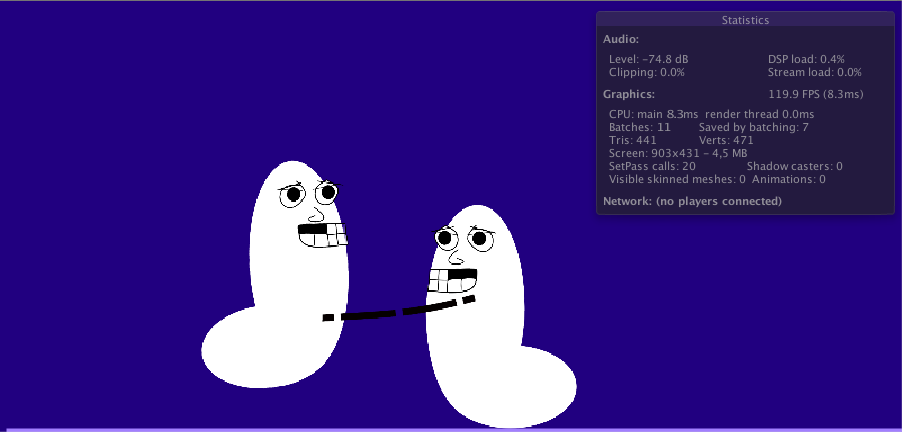
\includegraphics[width=0.7\hsize]{fig/attack}
\caption{Główne menu\label{RYS.2}}
\source{Opracowanie własne}
\end{figure}

\section{Wykorzystanie sztucznej inteligencji}
Nauczanie maszynowe dzieli się na kilka podstawowych typów. Są to:
\begin{enumerate}
\item Analityczne myślenie -- polega na wprowadzaniu dużej ilości oznakowanych
danych często z~opisanymi
parametrami i~wymuszanie nauki na ich podstawie. W~tym modelu komputer
podczas nauczania
poszukuje zależności i~połączeń pomiędzy wprowadzanym danym. Następnie
relacje są nałożone na
dołączone parametry. Przykładem takich implementacji są sieci
neuronowe.
\item Nienadzorowana nauka -- w~tym przypadku dane są nieoznakowane. Model taki wykorzystuje się do poszukiwania wzorów lub ulepszania już istniejących. 
Przykładem takiego algorytmu jest ,,k--means clustering''.
\item Zasilanie -- metoda ta pozwala na naukę poprzez obserwacje. Głównie
polega na interakcji z
otoczeniem i~wycenianiu stosunku ryzyka do nagrody. Taka nauka rozwija
umiejętności sztucznej
inteligencji w~sposób iteracyjny na zasadzie akcja--reakcja. Taka
implementacja jest stosowana głównie
do wyspecjalizowania rozwiązania do specyficznych warunków. Problem
 ,,Reinforcment Learning'' jest
uznawany za oddzielny problem w~dziedzinie algorytmów i~aktywnie
rozwijany. Właśnie ten typ
nauczania jest eksploatowany w~branży gier wideo i~uznawany jako
przyszłościowy. Główne etapy tego
algorytmu można podzielić na następujące punkty:
\begin{enumerate}
\item Obserwacja
\item Decyzja i~akcja
\item Nagroda i~kara
\item Wnioski
\end{enumerate}
Popularnymi algorytmami stosującymi zasilanie jest Q--learning lub
 ,,Temporal Difference (TD)''.
\end{enumerate}
Wybór modelu powinien być zależny od problemu. Algorytmy nadzorowane
wymagają dużej ilości
danych startowych, by rozpocząć naukę. Przy braku takowych warto
zastanowić się nad algorytmami
zasilanymi. Wymagają one jednak interaktywnego środowiska. Określonych
systemów nagradzania i~karania. Gdy problem nie spełnia takich wymagań, pozostają algorytmy
nienadzorowane, które pomagają
przy dużych ilościach danych nieopisanych lub gdy poszukiwane są
modele/wzorce.

Rozwój umiejętności awatara polega na wykorzystaniu utworzonych rankingów i~ciągłym
odświeżaniu pozycji ataków na liście poprzez obserwacje.
Czynnikiem decydującym o~wartościowaniu ataków jest różnica
pomiędzy dysproporcją kontroli nad postaciami przed i~po ich wykonaniu.
Gdy wartość ataku zostanie ponownie obliczona poprzez wykorzystanie
średniej arytmetycznej z~nowej i~starej wartości, zostanie on ponownie
umiejscowiony w~rankingu.
Dzięki systemowi ,,Echo'', ten sam atak, zależnie w~którym rankingu się
znajduje, może mieć inną pozycję w~rankingu. Pozwala to sztucznej
inteligencji na samodzielne wyspecjalizowanie wyuczonego ataku na
poszczególne sytuacje. W~przypadku braku ataku dla danej sytuacji,
wybierany jest atak eksperymentalny z~innych rankingów.
Przeciwnie do wykonywania ataków przez komputer, które odbywają się w~głównej
pętli, obserwacja jest wykonywania równolegle do głównego wątku gry.
Współbieżnie działają także aktualizowanie, dodawanie i~wybieranie ataków
przez system gry. Priorytetyzacja wykonywania ataków przez system
na równi z~graczem i~delegowanie mocniej obciążających prace procesora
zadań na współbieżne wątki zapewnia nie tylko płynność rozgrywki, ale
także daje gwarancje dynamicznego i~reaktywnego
pojedynku.
Taka implementacja systemu kontroli awatara niesie ze sobą ciekawe korzyści i~pozytywne cechy.
Przeciwnik będzie posiadać tylko te ataki, które zostaną zaobserwowane u użytkownika.
Sprowadza to zaistniałą sytuację do pozycji ,,mistrz--uczeń''. Wymiana
wiedzy pomiędzy graczem a~sztuczną inteligencją jest tutaj ściśle
powiązana z~tym, jakie umiejętności posiada żywy uczestnik walki. Ważne jest,
że mechanika ta nie implikuje bezpośrednio sytuacji, w~której przeciwny awatar nigdy nie
przekroczy umiejętności gracza. Dzięki rozwijanej umiejętności
dobierania coraz lepiej ataków do zaistniałej
sytuacji może dojść do momentu, w~którym system gry będzie lepiej
dostosowywało się niż użytkownik.
Ze względu na to, że przeciwnik jest wyspecjalizowany do
pojedynkowania z~poszczególnym użytkownikiem, program została zaprojektowana tak,
by wymiana plików z~zapisanymi umiejętnościami pomiędzy użytkownikami była
możliwie najłatwiejsza. Dzięki temu gracze mogą łączyć się w~grupy i
trenować swoje awatary nawzajem. Elementy angażujące wymianę doświadczenia z
graczami nie tylko werbalnie, ale też fizycznie jest ważnym elementem
utrzymania popularności gry, który jest coraz
częściej doceniany przez różne firmy. Wspomniane ułatwienie wymiany
danych odbywa się poprzez sprowadzenie całej lokalnej logiki sterowania awatarem przeciwnika w grze do dwóch
plików posiadających zoptymalizowane dane, który
jest łatwy w~odczytywaniu i~zapisywaniu przez system. Co więcej,
 ,,sztucznych inteligencji'' albo ,,przeciwników'' gracz może posiadać wiele i
w opcjach dokonujemy aktualnej konfiguracji. Wszystko to by wspierać
łączące się grupy.
Rankingi i~turnieje wyuczonych zawodników przez użytkowników na serwerach
online to tylko kilka dodatkowych propozycji na rozwój.
Powodem wyboru systemu polegającego na obliczaniu różnicy kontroli nad
postaciami jest prosty do obserwacji i
daje wymierne korzyści. Natomiast sama mechanika pozycjonowania ataków w
rankingach może zostać połączona z~innymi pomysłami. Na przykład dzięki
neuroewolucji, postać mogłoby dobierać następne ataki względem dokonanych
przed chwilą decyzji, a~nie na stałe względem panującej sytuacji.
\begin{figure}[!tbh]
\centering
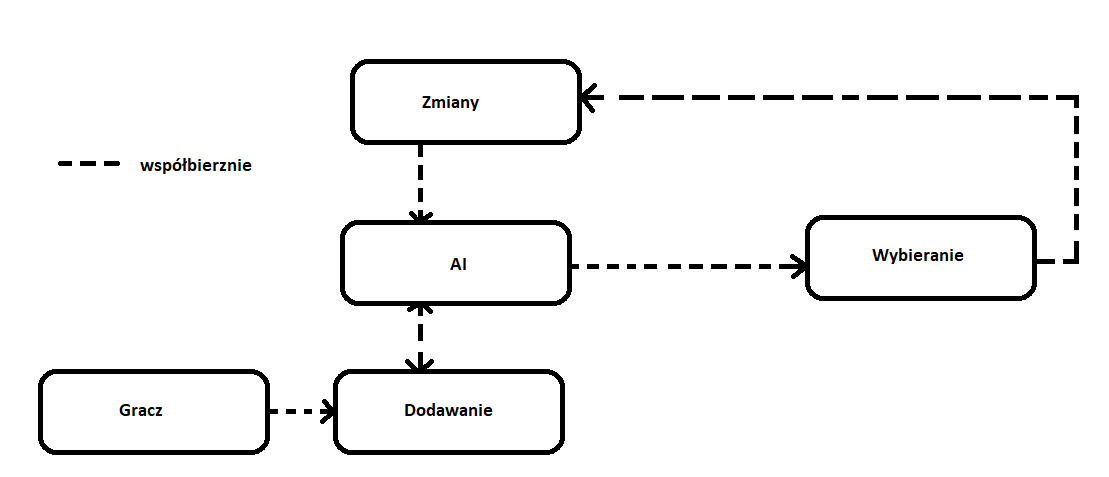
\includegraphics[width=0.7\hsize]{fig/echoFlow}
\caption{Ogólna logika gry\label{RYS.3}}
\source{Opracowanie własne}
\end{figure}

\begin{figure}[!tbh]
\centering
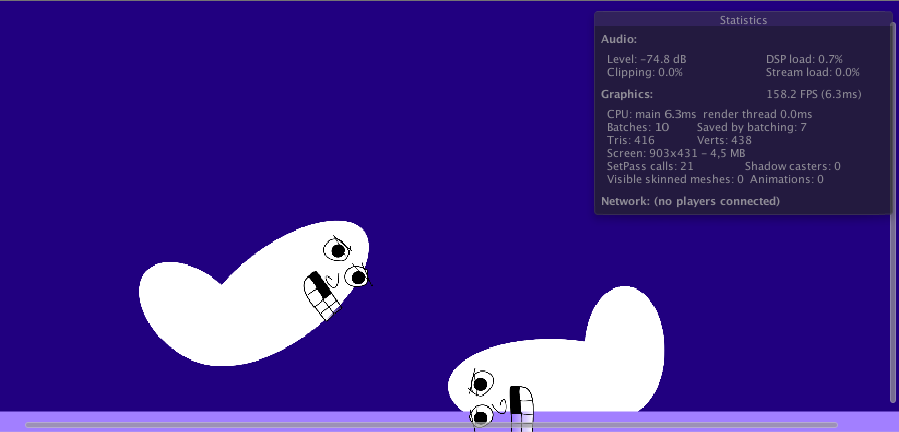
\includegraphics[width=0.7\hsize]{fig/knocked}
\caption{Główne menu\label{RYS.4}}
\source{Opracowanie własne}
\end{figure}
\section{Rankingi Echo}
System Echo określa w~jaki sposób ataki gracza są zapisywane do
rankingów. Po pierwsze awatar przeciwnika podczas nasłuchiwania obserwuje warunki
panujące na obszarze gry. Na warunki takie składają się:
\begin{enumerate}
\item Odległość pomiędzy awatarami
\item Kąt pomiędzy awatarami
\item Różnica wektora kontroli pomiędzy awatarami
\end{enumerate}
Panujące warunki w grze są obserwowane przez system, a~następnie
konwertowane do rozumianych przez awatara parametrów. System podczas zapisywania bierze pod uwagę wszystkie te rankingi, których choć jeden z~warunków
pasuje do panujących aktualnie. Powoduje to rozproszenie jednego ataku na
wiele różnych sytuacji, dzięki czemu taki ruch może osiągać lepsze wyniki
ze względu na wybraną ścieżkę
dostępu. Podczas zapisu atak jest zapisywany na odpowiedniej pozycji w
liście w~każdej ze ścieżek ze względu na osiągnięty wynik, czyli ilość
zadanych obrażeń minus ilość otrzymanych obrażeń podczas jego
wykonywania.
Na przykład dla $odległości = 1, kąt = 2, życie = 3$ można zaobserwować
poniższą sytuację przy dodawaniu nowego ataku:
\begin{minted}{csharp}
RankEcho[odległość=1][kąt=dowolnie][życie=dowolnie] = Add(combo1)
RankEcho[odległość=dowolnie][kąt=2][życie=dowolnie] = Add(combo1)
RankEcho[odległość=dowolnie][kąt=dowolnie][życie=3] = Add(combo1)
\end{minted}
\begin{figure}[!tbh]
\centering
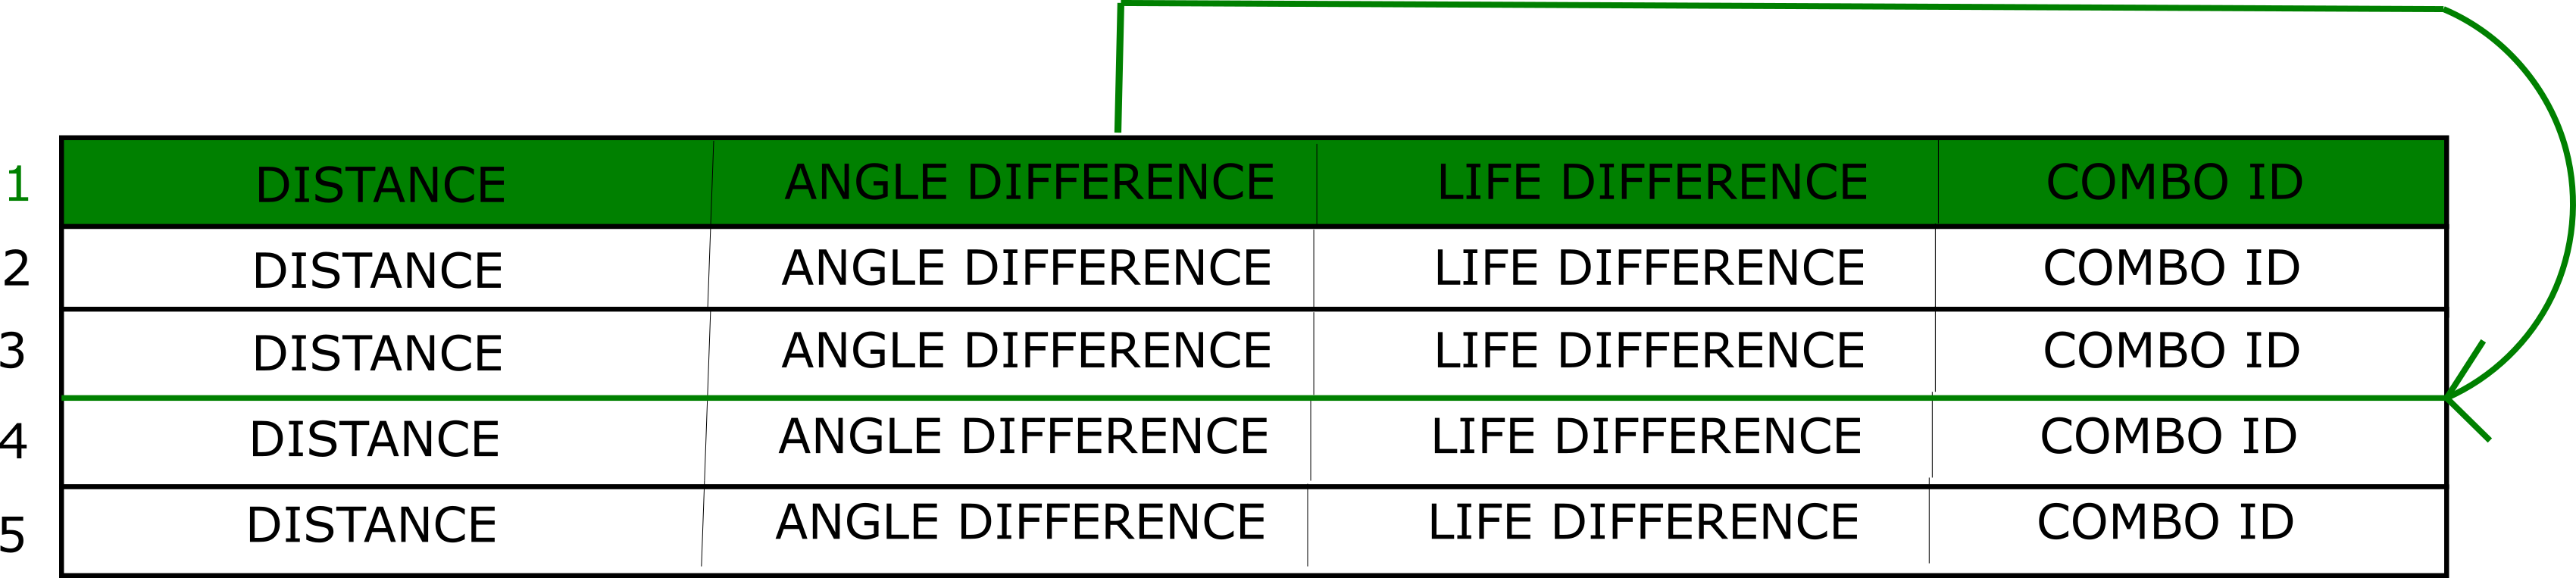
\includegraphics[width=.8\hsize]{fig/echoRankExample}
\caption{Schemat rankingu\label{RYS.5}}
\source{Opracowanie własne}
\end{figure}
Przy wyborze ataku przez awatar przeciwnika mamy natomiast sytuacje, w
której otrzymujemy tylko jeden konkretny ranking:
RankEcho[odległość=1][kąt=2][życie=3] = GetElement(0)
Przy wybieraniu ataku, to pierwszy z~listy w~wybranym rankingu zostaje
wybrany, ponieważ jest to atak z~najwyżej ocenionym wynikiem.

Rankingi Echo zostały zaimplementowane jako tablice pseudo--SQL z~czterema
kolumnami. Pierwsze trzy kolumny służą jako opis sytuacji, natomiast
ostatnia kolumna jest to lista z~ustaloną kolejnością,
posiadająca zapisane ID ataków. Dane te służą następnie do weryfikacji
ataku z~zmiennej typu ,,Dictionary'' posiadającej wszystkie ataki.
Konstrukcja ta pozwala na tworzenie zapytań SQL względem
panującej sytuacji i~uzyskania szybkiego dostępu do szeregu rankingów lub
jednego konkretnego, w~zależności od intencji. Przy uzyskaniu
poszukiwanego ID ataku, wykorzystujemy go, by uzyskać dostęp
do jego parametrów w~czasie O(1). Natomiast głównym powodem zastosowania
listy w~rankingach zamiast standardowej tablicy jest większa prędkość, z
jaką komputer radzi sobie ze zmianą rozmiaru wybranego typu względem
odrzuconych.
Pseudokod implementacji rankingu ,,Echo'':
\begin{minted}{csharp}
GetCombo ():
	sql = Select * from Echo where
		rememberedSituation1 = situationNow1 OR
		rememberedSituation2 = situationNow2 OR
		...
	EchoTemp = Echo.Find(sql)
	for i=0 to EchoTemp.Count do
		chosenCombo = max(EchoTemp[i], chosenCombo);
	end
	return chosenCombo;
end


AddCombo (newCombo):
	sql = Select * from Echo where
		rememberedSituation1 = situationNow1 OR
		rememberedSituation2 = situationNow2 OR
		...
	EchoTemp = Echo.Find(sql)
	for i=0 to EchoTemp.Count do
		EchoTemp[i].Add(newCombo)
	end
end

ChangeCombo (oldCombo, j):
	EchoTemp[j].Replace(oldCombo)
end
\end{minted}
\section{Sterowanie i~menu}
Podczas działania gry, zarówno w~menu jak i~podczas walki, w~celu
dołączenia i~przejęcia kontroli nad drugim awatarem przez drugiego
gracza, musi zostać naciśnięty przycisk ,,start'' na drugim podłączonym
kontrolerze. System kontrolujący postacią przeciwnika zostanie natychmiast wyłączone aż do następnego
przyciśnięcia ,,start'' na tym samym kontrolerze. Gdy tak się stanie,
sytuacja powraca do poprzedniego stanu, gdzie komputer przejmuje kontrole nad postacią przeciwnika i
bierze udział zarówno w~walce jak i~nabieraniu doświadczenia.

Każda z~postaci ma dwa ośrodki kontroli. Jeden umiejscowiony na wysokości
twarzy. Odpowiada on za kontrole nad górną
częścią ciała. Odnosi się to zarówno do odchylania się jak i~atakowania
rękoma. Drugi ośrodek znajduje się w~dolnej części ciała, na wysokości
ogona. Odpowiada on za przemieszczanie się tej części ciała i~za
kopnięcia. Zadane obrażenie w~daną część ciała obniża kontrole nad
odpowiednim ośrodkiem. Im mniejsza kontrola, tym wolniejsza reakcja i
mniej zadawane obrażenia. Co więcej, gdy suma kontroli nad ośrodkami
wynosi poniżej 5 procent, dana postać nie będzie w~stanie się podnieść po
upadku. Podczas poruszania się, postać może upaść. Upadek oznacza
sytuacje, w~której dana postać znajduje
się na ziemi, a~jej odchył przekroczył dozwoloną ilość stopni. W~takiej
sytuacji, dopóki gracz nie wykona akcji podnoszenia, nie może wykonywać
żadnych innych ruchów. Im szybciej, tym lepiej,
ponieważ leżąca postać, nie mogąc się bronić, jest wystawiona na ataki
przeciwnika. Powoduje to sytuacje, w~której kontrola nad rotacją awatara zarówno na ziemi jak i~powietrzu, jest kluczowa dla dobrej walki. Wyskoki to ważny element gry. Przy dobrze
wyuczonej obronie, walka na ziemi może nie wystarczyć. Z~pomocą dochodzi umiejętność walki w~powietrzu. Skok może być niski,
zainicjalizowany za pomocą tylko jednego
analoga, albo wysoki, z~dwoma analogami. Im mniejsza kontrola nad
postacią, tym mniejsze skoki. Podczas skakania postać może obracać się bez
ograniczeń. Przy odpowiednich umiejętnościach, gracz,
za pomocą odpowiednio dobranych ruchów może znaleźć się za plecami przeciwnika, zadając wiele obrażeń po drodze. Dodatkowo, postać może
uzyskać zwiększoną moc wyskoku poprzez trzymanie jednego lub
obu analogów (zależnie do którego rodzaju skoku) w~dół. Jednak jeśli skok
nie nastąpi po ładowaniu, wartość bonusu drastycznie maleje do zera.
Wspomniane ośrodki odgrywają główną rolę w~poruszaniu się na ziemi. Na
podstawie animacji postaci przeciwnika, gracz może spodziewać się ataków
na odpowiednich wysokościach (góra/środek/dół). W
odpowiedzi można odchylić górną część ciała lub przemieścić dolną w~celu
uniknięcia ataku. Jeśli brakuje czasu, drugą opcją jest obrona. Użytkownik
nadal musi wybrać wysokość, na której będzie się bronić, jednak
tym razem reakcja postaci jest niemal natychmiastowa. Minusem tego
rozwiązania jest to, że nadal część obrażeń jest rozprowadzona równomiernie na oba ośrodki ciała.
Postać może się bronić na dwa sposoby. Poprzez blokowanie ataków z góry, lub te wycelowane na środku wysokości awatara. W~przypadku tych ostatnich, postać obroni atak niezależnie od
wysokości, jednak otrzymane obrażenia będą tylko
nieznacznie ograniczone. Wyjątkiem są ataki na wysokości środka. W~takim
razie obrażenia są ograniczone tak samo, jak w~przypadku pasującej obrony
góry i~ataku na tejże wysokości. Lewy trigger
odpowiada za obronę lewej ręki i~lewej nogi, natomiast prawy trigger
prawą ręką i~lewą ręką. Pozycja obrony jest determinowana na podstawie
wciśniętych ,,triggerów''. W~zależności czy strona obrony (prawa lub lewa)
pasuje do strony ataku, obrażenia z~ataku zostaną odpowiednio
zredukowane. Jeśli nie pasuje, obrażenia zostaną w~pełni zadane drugiemu
awatarowi. Obronę można wykonywać obustronnie na raz.
Do dyspozycji gracza zostały oddane cztery ataki. Lewa i~prawa pięść oraz
lewe i~prawe kopnięcie. Jednak awatar może wykonywać tylko jedną akcję
ataku na raz. Dodatkowo blok blokuje postać przed wykonywaniem
którejkolwiek z~tych czterech akcji. Jednak podczas wykonywania takiej 
akcji, postać może jednak dowolnie się przemieszczać i~skakać, jednak
prędkość i~wysokość jest zmniejszona. Input, jaki jest wprowadzany przez system ma dokładnie taką samą strukturę jak input użytkownika
dzięki strukturze zapisywanych danych. Tak samo
obserwacja, jaką wykonuje program na rzecz postaci przeciwnika dokonywana jest tylko na
podstawie wizualnych efektów, jak odległość czy różnica kątów. Dzięki temu
użytkownik może mieć poczucie wyrównanych szans i~braku faworyzowania przeciwników
co jest częstym problemem w~innych grach, szczególnie akcji, jak i strategicznych. Oprogramowanie wspiera wszystkie kontrolery posiadające dwa analogi, cztery
przyciski i~dwa triggery. Oznacza to, że do grania użytkownik musi posiadać
urządzenie z~opisaną powyżej
specyfikacją.

Sterowanie dla kontrolera XBOX i~PlayStation 3:
\begin{itemize}
\item Kontrola dół -- lewy analog
\item Kontrola góra -- prawy analog
\item Lewa pięść -- X
\item Prawa pięść -- B
\item Lewa noga -- Y
\item Prawa noga -- A
\item Lewa obrona -- lewy trigger
\item Prawa obrona -- prawy trigger
\item Skok -- analog.y > 0.5
\item Wysoki skok -- analogi.y > 0.5
\item Wstawanie -- analog.y > 0
\item Ładowanie skoku -- analog.y < 0
\item Przemieszczanie w~lewo -- analogi.x<0
\item Przemieszczanie w~prawo -- analogi.x>0
\item Rotacja w~powietrzu w~lewo -- analog1.x > 0 and analog2.x < 0
\item Rotacja w~powietrzu w~prawo -- analog1.x < 0 and analog2.x > 0
\end{itemize}
Rozgrywka została zaprojektowana tak, by gracz od razu przenosił się do
pojedynku. Jeśli naciśnie
jakikolwiek przycisk gra rozpocznie odliczanie i~rozpocznie się rozgrywka z
domyślnie włączoną sztuczną inteligencją, która od razu zacznie sterować
drugim awatarem. Wykryta aktywność na drugim
kontrolerze spowoduje wyłączenie systemu kontrolującego postacią przeciwnika i~kontrola nad drugim awatarem
zostanie do niej przydzielona.
Menu można przywołać za pomocą przycisku start na kontrolerze. Menu
zatrzyma czas aktualnie rozgrywanej sesji oraz oferuje do wyboru:
\begin{itemize}
\item Resume -- powrót do trwającej walki
\item Options -- opcje gry. Tutaj użytkownik może zmienić muzykę odgrywaną podczas rozgrywek na
swoją własną za pomocą przycisku ,,Change game music'', może także zmienić
tło gry za pomocą przycisku ,,Change background''. Wszystkie opcje zmuszają użytkownika do
wybrania odpowiedniego pliku. Po dokonaniu wyboru użytkownik powraca do
wyboru w~zakładce ,,Options'' z~odświeżonym stanem gry. Natomiast ostatnim
przyciskiem jest opcja ,,Back'', który powraca gracza do głównego menu.
\item Quit -- nadpisuje nową logikę dla awatara w~odpowiednim pliku i~wyłącza
program
\item Quit without save -- wyłącza program bez nadpisywania nowej logiki

\end{itemize}
\begin{figure}[!tbh]
\centering
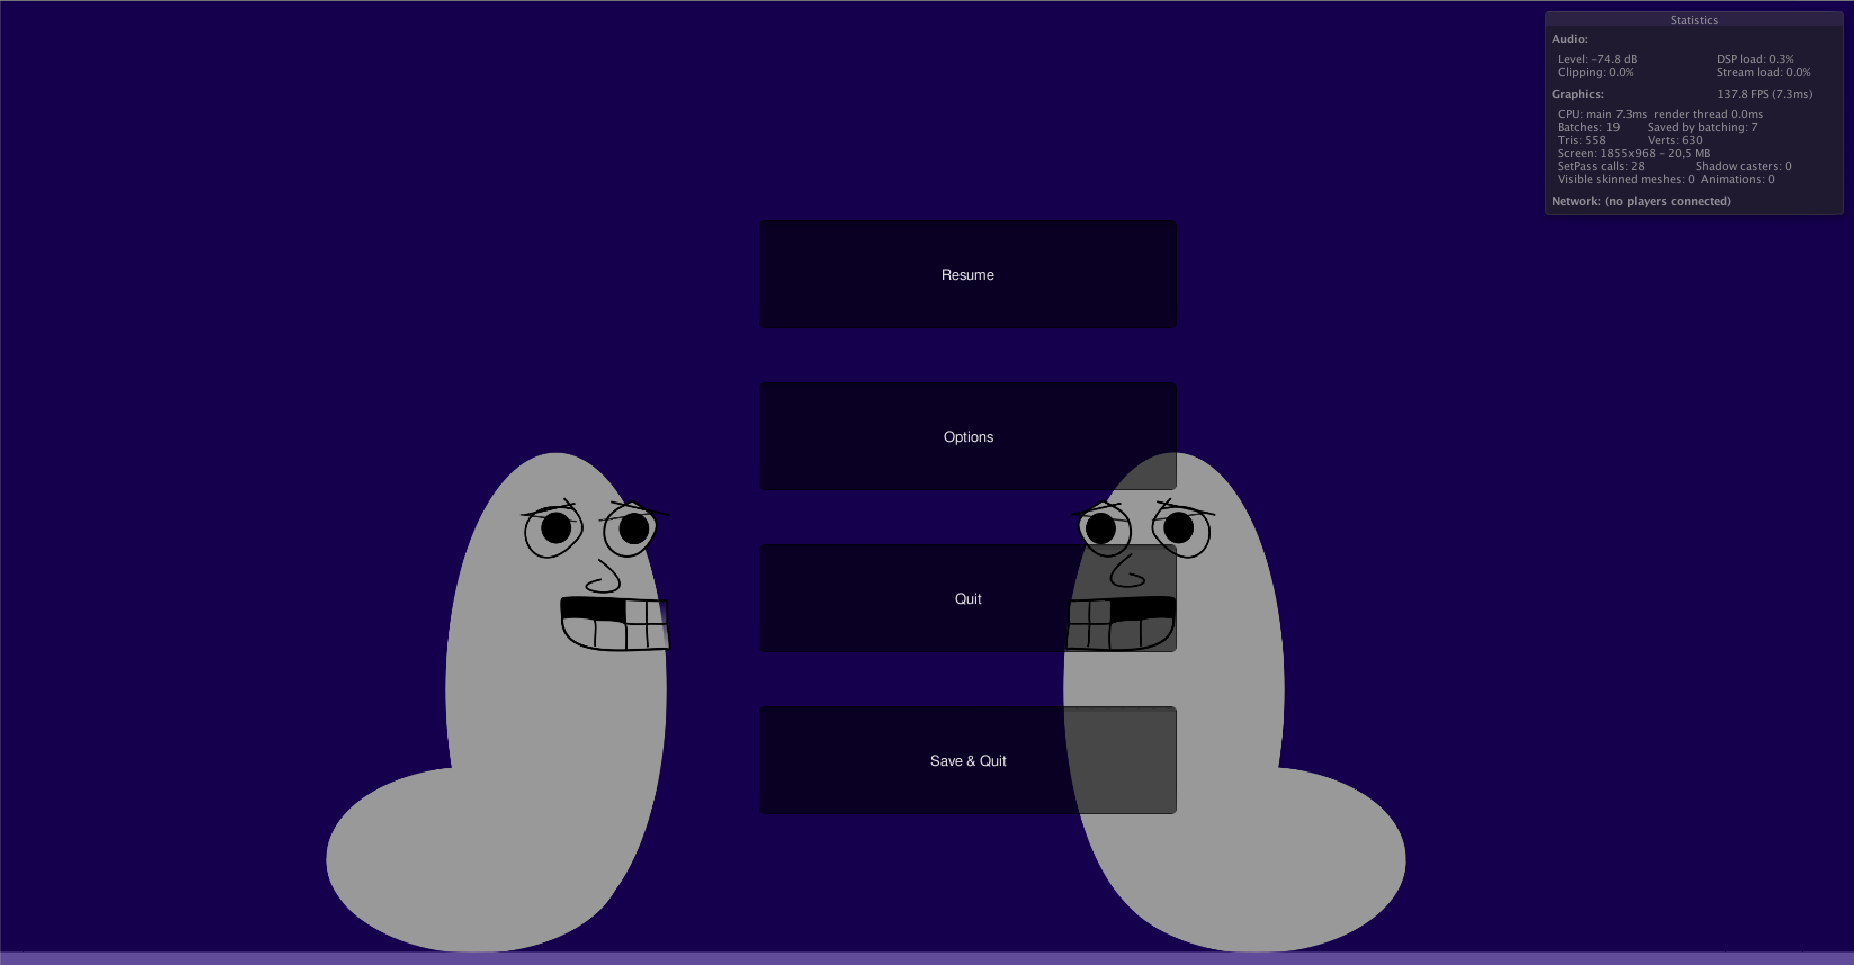
\includegraphics[width=0.7\hsize]{fig/menu1}
\caption{Główne menu\label{RYS.6}}
\source{Opracowanie własne}
\end{figure}
\begin{figure}[!tbh]
\centering
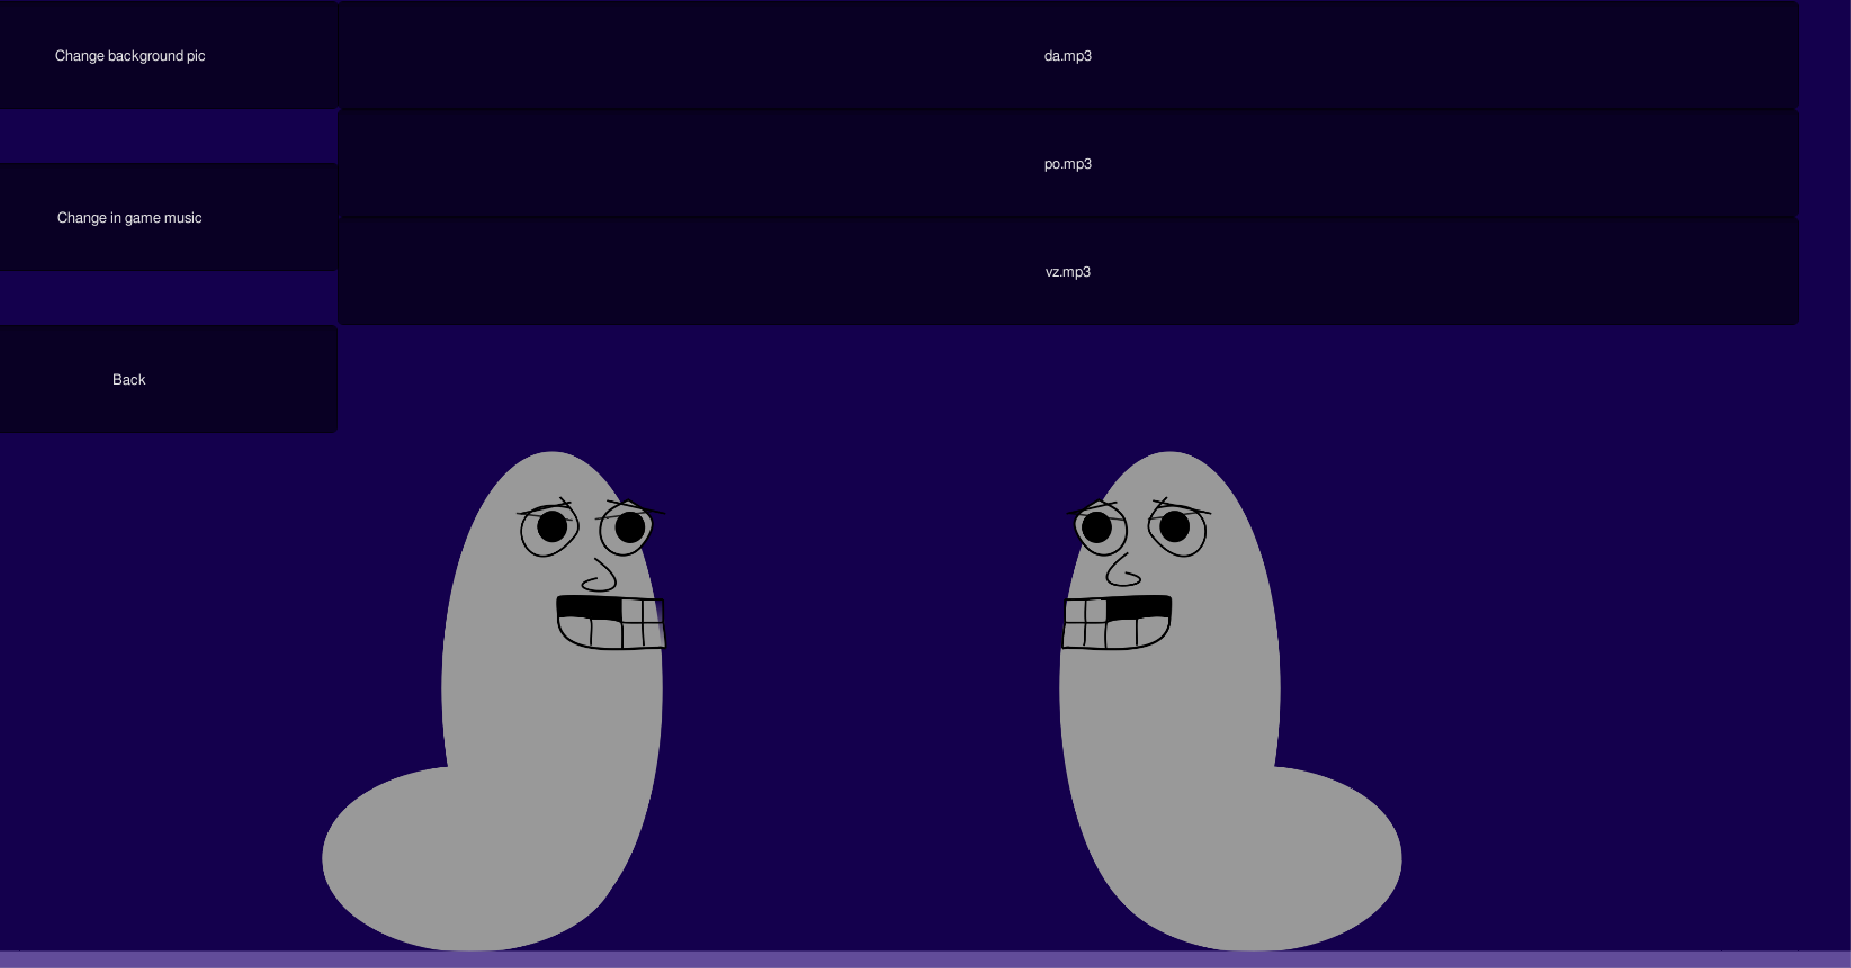
\includegraphics[width=0.7\hsize]{fig/menu2}
\caption{Opcje wybieranie plików\label{RYS.7}}
\source{Opracowanie własne}
\end{figure}

% zakończenie
\summary
Cały projekt miał za zadanie umożliwienie trenowania własnego
przeciwnika. Awatar zdobywa
umiejętności powoli, czego można się było spodziewać. Same walki z~nim
bywają ciekawe i~zróżnicowane. Wbudowane menu, balans postacią i~charakterystyczne
sterowanie może być inspiracją
do następnych projektów. Dynamicznie rozwijający się silnik Unity3D i występujące problemy z kompatybilnością z systemem Ubuntu prowadził do spowolnienia procesu deweloperskiego. Gra umożliwia także na pojedynki dla dwóch graczy, które można traktować jako oddzielny tryb rozgrywek, umożliwiający sesje dla znajomych, jak i kompetytywne turnieje. Gra będzie
udostępniona na szeregu różnych platformach udostępniających oprogramowanie zarówno na konsole jak i~komputery na najpopularniejszych systemach operacyjnych w~tym Windows, OSX i~Ubuntu. 
% załączniki (opcjonalnie):
\appendix

\chapter{Gra ,,Fighty''}
Spakowany plik z~grą i~wszystkimi potrzebnymi plikami do poprawnego
działania na nośniku USB.


\begin{document}

\end{document}
\section*{Słownik}
%\chapter{Słownik}
\label{slownik}
\begin{itemize}
\item CO--OP -- skrót z angielskiego od ,,cooperation'', oznacza gry z mechaniką zaprojektowaną do rozgrywki dla bardzo małej ilości osób naraz.

\item Joint -- łącznik, mechanizm popularny w silnikach z symulacją fizyki, pomagający wyznaczyć wzajemny wpływ danych obiektów na siebie.

\item FPS -- skrót z angielskiego od ,,frames per second'', oznacza ilość klatek na sekundę. Jest to główny wyznacznik płynności gry na danym sprzęcie. Na przykład, dla konsol, akceptowalna minimalna ilość klatek na sekundę to 30, a~na komputerach 60. Natomiast standardem w branży filmowej to średnio 24 klatek na sekundę.


\item Awatar -- przedstawiciel gracza w wirtualnym świecie. W grze jest to postać, nad którą użytkownik lub system gry ma kontrolę.

\end{itemize}
% literatura (obowiązkowo):
\begin{bibdiv}
\begin{biblist}
\label{bib}
\bib{Video games history}{article}{
title={Dokumentacja Unity3D},
date={2018},
pages={https://docs.unity3d.com/ScriptReference/GUI.BeginScrollView.html}
}
\bib{AI}{article}{

title={Rozważania nad sztuczną inteligencją},
date={2018},
pages={https://www.ted.com/topics/ai},}
\bib{history}{article}{
title={Historia gier wideo},
date={06.2018},
pages={https://en.wikipedia.org/wiki/History\_of\_video\_games},}
\bib{machine}{article}{
title={Nauczanie maszynowe},
date={2018},
pages={https://en.wikipedia.org/wiki/Machine\_learning},}

\bib{Ray Tracing}{article}{
title={Turner Whitted ,,Multi--bounce Recursive Ray Tracing},
date={1979},
pages={},}



\end{biblist}
\end{bibdiv}

% spis tabel (jeżeli jest potrzebny):
\listoftables
% spis rysunków (jeżeli jest potrzebny):
\listoffigures
\oswiadczenie
\end{document}